\chapter{Data and Experimental Setup} \label{chap:setup}

\section{Training, Calibration, and Testing}

\subsection{Data Construction} \label{sec:data_construction}
The dataset comprises responses from candidates taking the Linguaskill exams for second language (L2) \nomenclature[Z]{L2}{Second Language} learners of English. These exams are divided into five sections, each scored on a scale from 0 to 6. This study focuses on Part 1, where candidates answer eight questions about themselves \cite{linguaskills}. Candidates are provided 10 seconds to respond to the first four, and 20 seconds for the last four. The first two questions are not graded. Overall, the candidates' performance across all sections is mapped to CEFR levels ranging from A1 to C2 \cite{CEFR}.

For text-based model, the dataset contains the response transcripts extracted from the audio files. For feature-based model, the dataset contains the 356-dimensional features extracted from the audio files. For audio-based model, the dataset contains the audio represented in vector format. Each item in the dataset has an associated candidate number to identify teh candidate, and the corresponding score from the human graders.

The dataset is divided into three sections: training, calibration, and testing. The training set is used to train the model, the calibration set is used to tune linear calibration after the score prediction from the neural network (Chapter \ref{chap:graders}), and the testing set is used to evaluate the model's performance. Table \ref{tab:data_size} shows the number of candidates in each section of the dataset.

\begin{table}[H]
    \centering
    \begin{tabular}{|c|c|c|}
        \hline
        \textbf{Training} & \textbf{Testing} & \textbf{Calibration} \\ \hline
        31471             & 1048             & 1033                 \\ \hline
    \end{tabular}
    \caption{Number of candidates in each section of the dataset}
    \label{tab:data_size}
\end{table}

The metadata about the candidates are also provided, including their age, gender, and first language. Based on the metadata, four distinct groups of concepts were identified: grades, categorized as $\leq$ A2 ($\leq$ 2.0), $\geq$ B2 ($\geq$ 4.0), and $\geq$ C1 ($\geq$ 5.0); first language, with Thai and Spanish chosen for the experiment; young candidates, defined as those aged $\leq$ 30; and male gender. The non-grade concepts are to test the model's output would not be affected by them, while the grade concepts are to test the opposite.

To verify that the dataset is unbiased, the average scores across the training, calibration, and testing sets were calculated for each group of concepts, shown in Table \ref{tab:avg_scores}. The scores for candidates having that concepts (+ve target) and not having that concepts (-ve target) are both included. Except for an outlying Thai -ve target score of 2.90 from the calibration set, the average scores for all non-grade concepts are within the range of 3.0 to 4.0, indicating a balanced distribution of scores across the dataset. The average scores for +ve target candidates from grade concepts are out of the range, with $\leq$ A2, $\geq$ B2, and $\geq$ C1 having average scores of 2.48, 4.29, and 5.15 respectively, which is expected based on the cutoff of the CEFR levels. It could be concluded that the dataset is not biased towards any specific group of candidates under consideration.

\begin{table}[H]
    \centering
    \begin{tabular}{|lc|c|c|c|c|c|c|c|}
        \hline
        \multicolumn{2}{|l|}{\textbf{}}                            & \textbf{\textless{}A2} & \textbf{\textgreater{}B2} & \textbf{\textgreater{}C1} & \textbf{Thai} & \textbf{Spanish} & \textbf{Male} & \textbf{Young}        \\ \hline
        \multicolumn{1}{|l|}{\multirow{2}{*}{\textbf{Training}}}   & \textbf{+ve target}    & 2.48                      & 4.29                      & 5.15          & 2.99             & 3.61          & 3.41           & 3.56 \\ \cline{2-9}
        \multicolumn{1}{|l|}{}                                     & \textbf{-ve target}    & 3.67                      & 3.19                      & 3.40          & 3.55             & 3.25          & 3.41           & 3.21 \\ \hline
        \multicolumn{1}{|l|}{\multirow{2}{*}{\textbf{Testing}}}    & \textbf{+ve target}    & 2.25                      & 4.54                      & 5.13          & 3.02             & 3.44          & 3.57           & 3.73 \\ \cline{2-9}
        \multicolumn{1}{|l|}{}                                     & \textbf{-ve target}    & 4.12                      & 2.88                      & 3.37          & 3.64             & 3.59          & 3.53           & 3.15 \\ \hline
        \multicolumn{1}{|l|}{\multirow{2}{*}{\textbf{Calbration}}} & \textbf{+ve target}    & 2.36                      & 4.46                      & 5.14          & 2.90             & 3.44          & 3.51           & 3.58 \\ \cline{2-9}
        \multicolumn{1}{|l|}{}                                     & \textbf{-ve target}    & 3.96                      & 2.97                      & 3.39          & 3.58             & 3.50          & 3.25           & 3.33 \\ \hline
    \end{tabular}
    \caption{Average scores for each type of concepts}
    \label{tab:avg_scores}
\end{table}

In addition, the percentage of positive targets for each concept from the training data is shown in Table \ref{tab:pos_target}, which would be used for the CAV extraction. This is useful for the comparison of the CAV performance with no weighting and balanced weighting. For a more skewed percentage, the use of balanced weighting would have a more significant effect on the CAV performance.

\begin{table}[H]
    \centering
    \begin{tabular}{|c|c|}
        \hline
        \textbf{Concept} & \textbf{\% of +ve} \\
        \hline
        $\geq$ C1        & 0.25               \\
        $\geq$ B2        & 19.7               \\
        $\leq$ A2        & 22.7               \\ \hline
        Thai             & 24.6               \\
        Spanish          & 44.8               \\ \hline
        Young            & 56.4               \\ \hline
        Male             & 47.6               \\
        \hline
    \end{tabular}
    \caption{Percentage of positive labelled data in training data}
    \label{tab:pos_target}
\end{table}


\subsection{Process of Training, Calibration, and Testing}

Figure \ref{fig:flow} illustrates the process requires to obtain the bias measurement with gradient distance. The grey boxes represents the main steps of the process, including model training and calibration, gradient and CAV extraction, and gradient distance measurement. The blue boxes represent the performance evaluation steps that could be done throughout the flow, including the model and the CAV accuracy. FInally, the dotted white boxes represent the data used in each step. To highlight, while the testing set is used for model evaluation, the training set is used for CAV evaluation. This choice is made as the CAV evaluation is to measure how accurately the CAV represents the concept during the training process itself.

\begin{figure}[H]
    \centering
    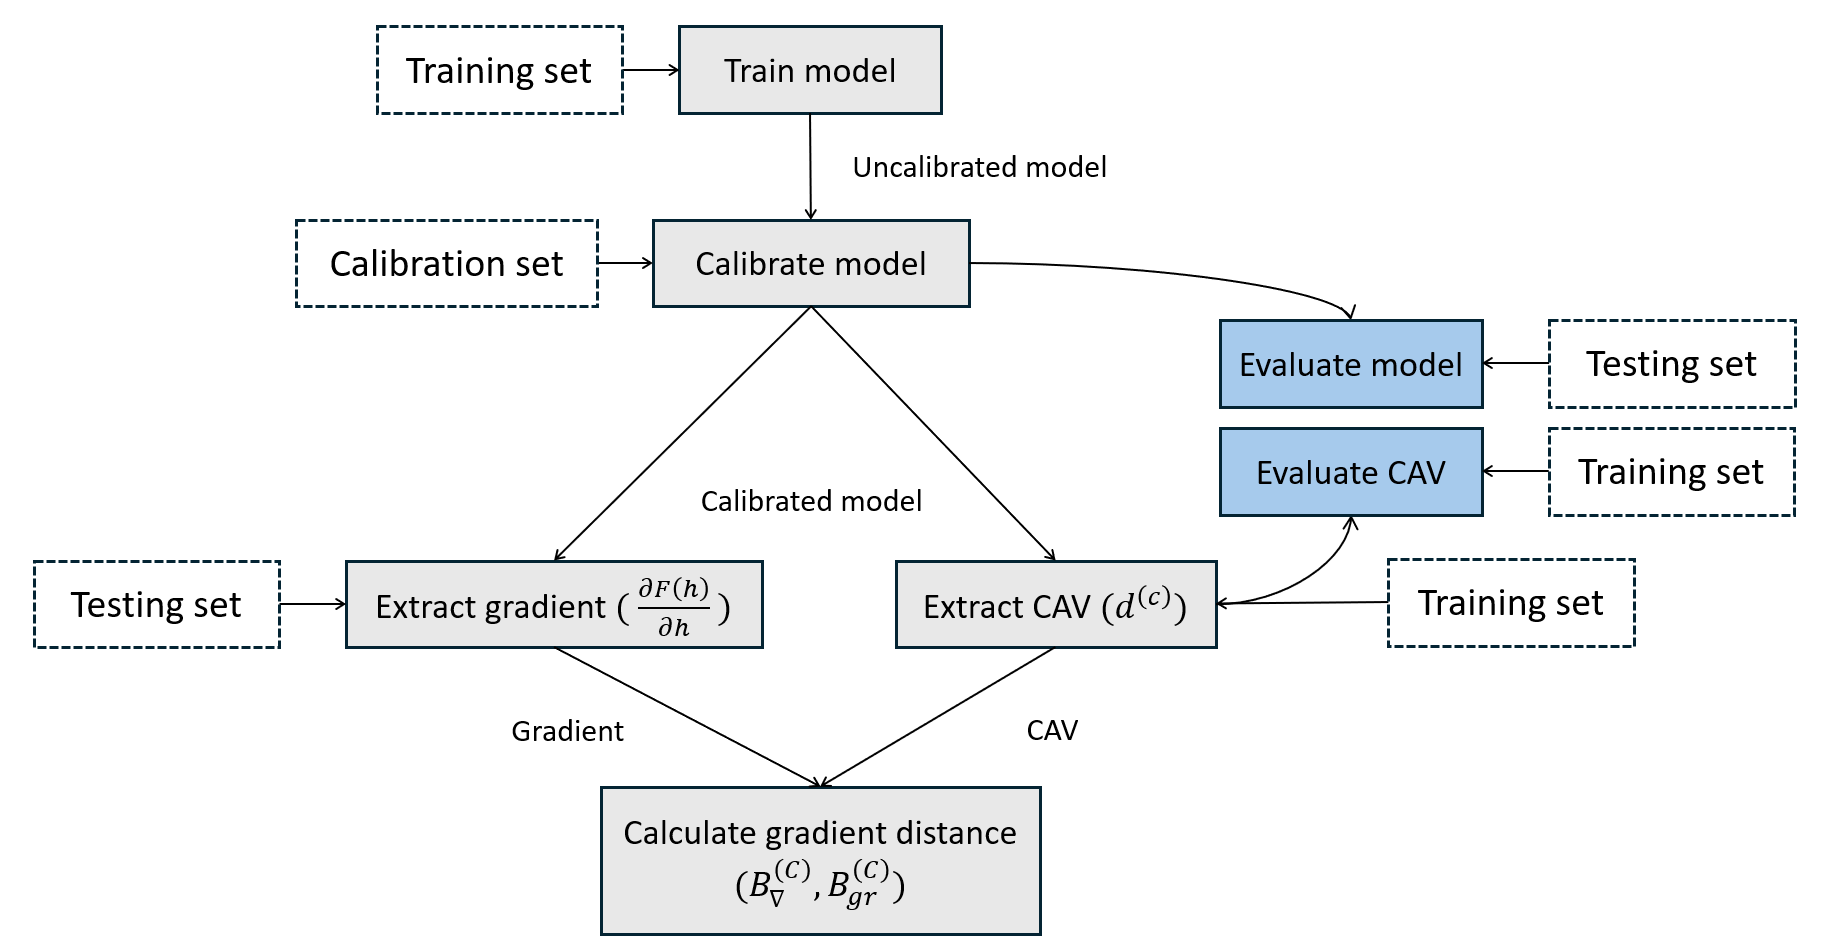
\includegraphics[width=0.95\textwidth]{flow.png}
    \caption{Flow of the process to obtain the bias measurement with gradient distance}
    \label{fig:flow}
\end{figure}

\section{Hyper-parameters}
\subsection{Model Training}
The architecture of the models used for training has been outlined in Chapter \ref{chap:graders}.

Ensemble seed

\subsection{CAV Linear Classifier Training}

\section{Model Biasing}

Adding 1 mark, maximum 6 marks to candidates related to the concept

\section{Factor Isolation}

Use of BERT-like architecture for feature model

Use of DNN instead of DDN for feature model

Deep fusion of feature and BERT attention

\section{Performance Criteria}
Model accuracy (what is RMSE, PCC, $<0.5$, $<1$)

CAV accuracy

Gradient distance for bias